\begin{center}
 \begin{minipage}[b]{0.45\textwidth} 
\subsubsection*{General information}
 Name: David Nikolaj Vinje \newline
 Address: Islands brygge 56b 1tv \newline
 Zip nr. 2300 Koebenhavn S \newline
 Phone number: 26325635 \newline
 E-mail: david2300@hotmail.com \newline
 Country: Danmark \newline
 Date of birth: 11/06/1995 
 \end{minipage}
 \hfill
\begin{minipage}[b]{3cm}
 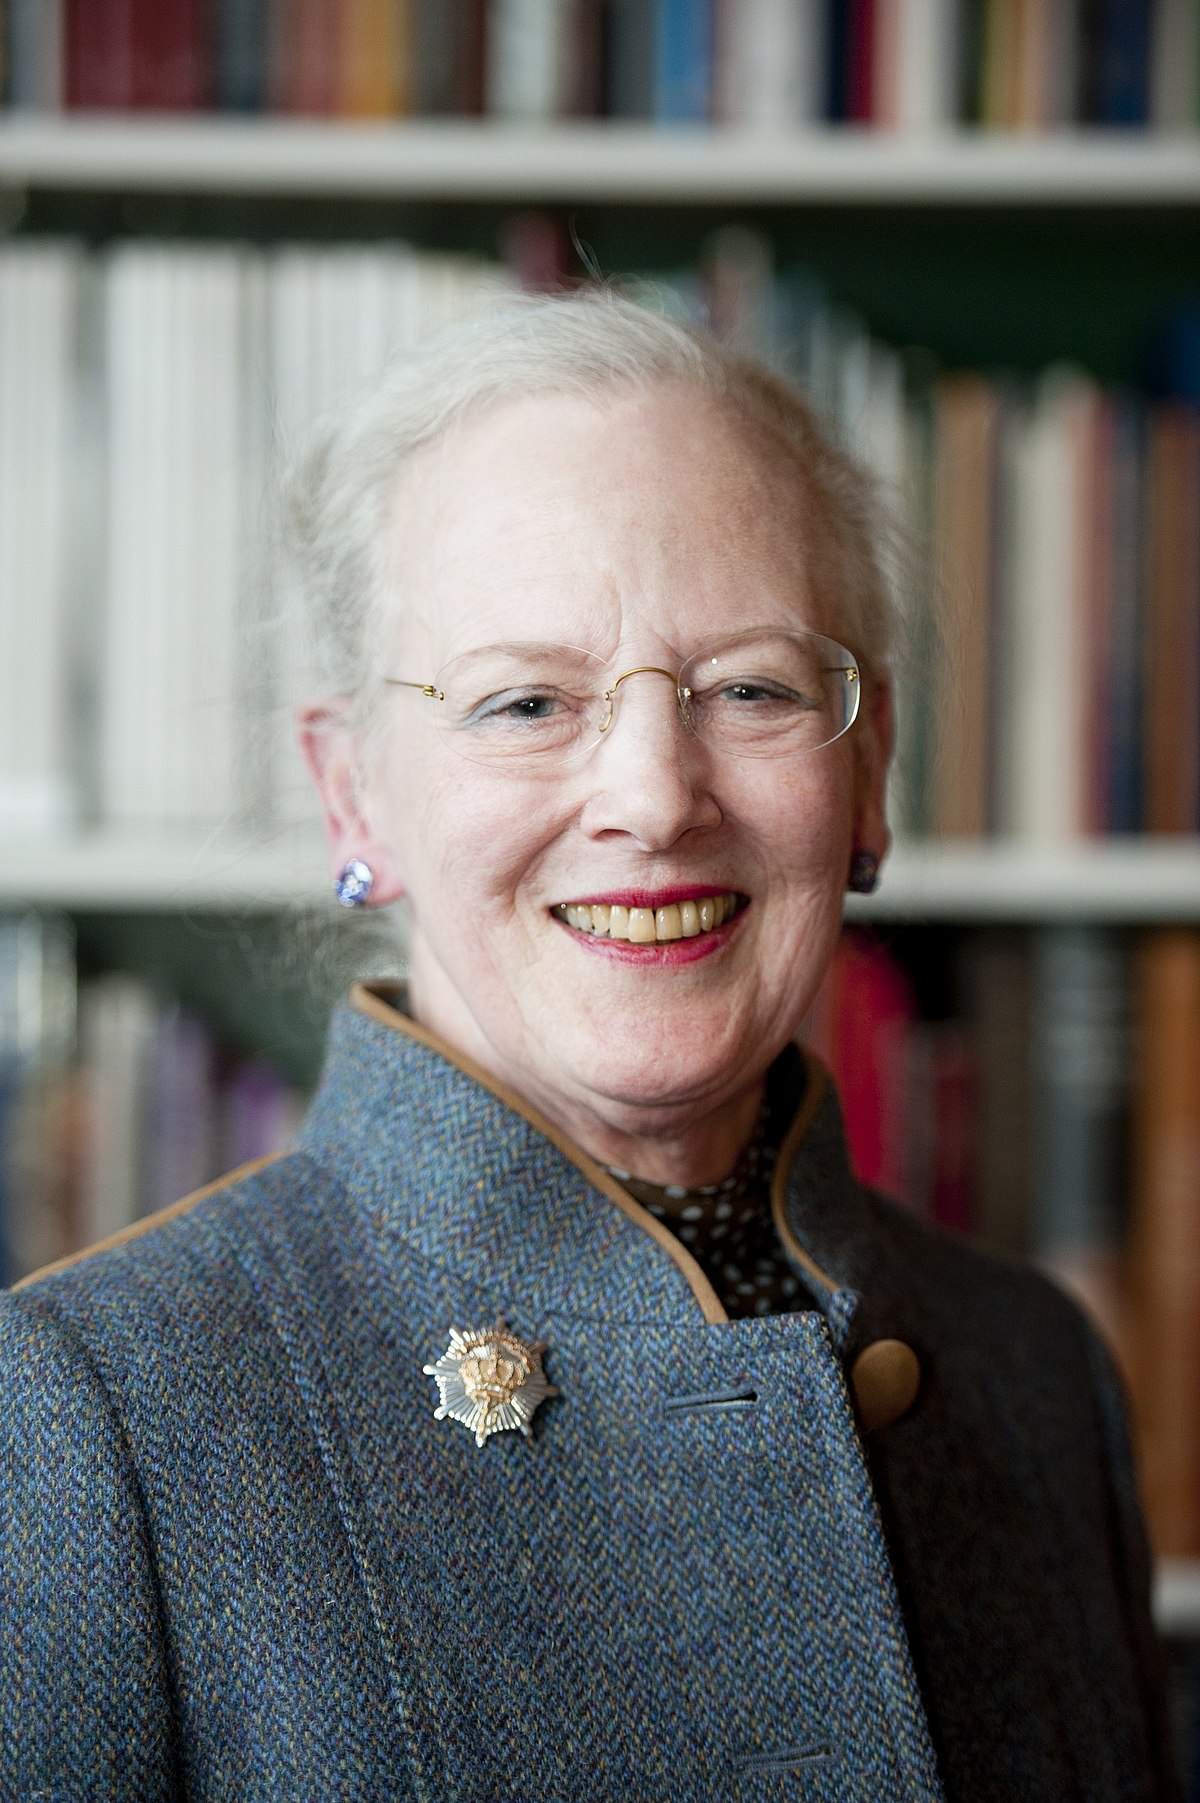
\includegraphics[height=4cm]{figures/1200px-Drottning_Margrethe_av_Danmark}
 \end{minipage}
 \end{center}

\section*{Free text}
Took a highschool diploma in Biotechnology and chemistry, where i ended with a grade of 10.7.
Took a highschool diploma in Biotechnology and chemistry: capable of doing PCR testing.
Highschool exam project was using c sharp (unity) to make a game.
Currently doing a bsc in engineering (software) at Aalborg university.
University focuses on teamwork, so i have lots of experience with larger groups.
Lots of skills in programming.
Large interest in electronics. Done multiple projects.
Capable of using machine learning using python. Also read a lot of statistics and probability theory to learn the theory behind it. Can use neural networks, to predict behavior.
Degree in computer science

